\documentclass{beamer}

\usepackage[utf8]{inputenc}
\usepackage[T1]{fontenc}
\usepackage{lmodern} % get rid of fontsize warning

\usepackage{tikz}
\usepackage{pgfplots}
\usepackage{verbatim}
\usepackage{amsmath}
\usepackage{textpos}
\usepackage{siunitx}
\usepackage{graphicx}
\usepackage[normalem]{ulem}


% for strings as xticks:
% see http://stackoverflow.com/questions/2908513/pgf-tikz-string-symbols-as-input-coordinates



\title{Simulating a Bunch of Galaxies for HETDEX}
\author{Henry~Gebhardt}
\institute{Department of Astronomy and Astrophysics,\\
The Pennsylvania State University}
\date{Astro 585 --- HPC and Astronomers?\\ April 23, 2014}
\titlegraphic{
\includegraphics[width=\textwidth]{logo_hetdex.jpg}}



\newcommand{\LAE}{Ly-$\alpha$ emitter}
\newcommand{\LAEs}{\LAE{}s }
\newcommand{\OIII}{{[}O{\sc III}{]}}
\newcommand{\OII}{{[}O{\sc II}{]}}
\newcommand{\NII}{{[}N{\sc II}{]}}
\newcommand{\NeIII}{{[}Ne{\sc III}{]}}
\newcommand{\Halpha}{H$\alpha$}
\newcommand{\Hbeta}{H$\beta$}
\newcommand{\Hgamma}{H$\gamma$}
\newcommand{\OIIIll}{\OIII4959,5007}
\newcommand{\OIIl}{\OII3727}
\newcommand{\NeIIIl}{\NeIII3869}
\newcommand{\NIIl}{\NII6583}
\newcommand{\Hbetal}{\Hbeta4861}
\newcommand{\Hgammal}{\Hgamma4340}

% journals
%\newcommand{\aap}{A\&A}
%\newcommand{\mnras}{MNRAS}

% units
%\DeclareSIUnit \solarmass {\ensuremath{\textrm{M}_{\odot}}}

\newcommand{\Msol}{\ensuremath{\text{M}_\odot}}
\newcommand{\Zsol}{\ensuremath{\text{Z}_\odot}}
\newcommand{\yr}{\ensuremath{\text{yr}}}
\newcommand{\erg}{\ensuremath{\text{erg}}}
\newcommand{\second}{\ensuremath{\text{s}}}
\newcommand{\kilometer}{\ensuremath{\text{km}}}
\newcommand{\angstrom}{\ensuremath{\text{\AA}}}


\begin{document}

\frame{\titlepage}

\frame{
    \frametitle{Hobby Eberly Telescope Dark Energy Experiment (HETDEX)}

    \begin{center}
        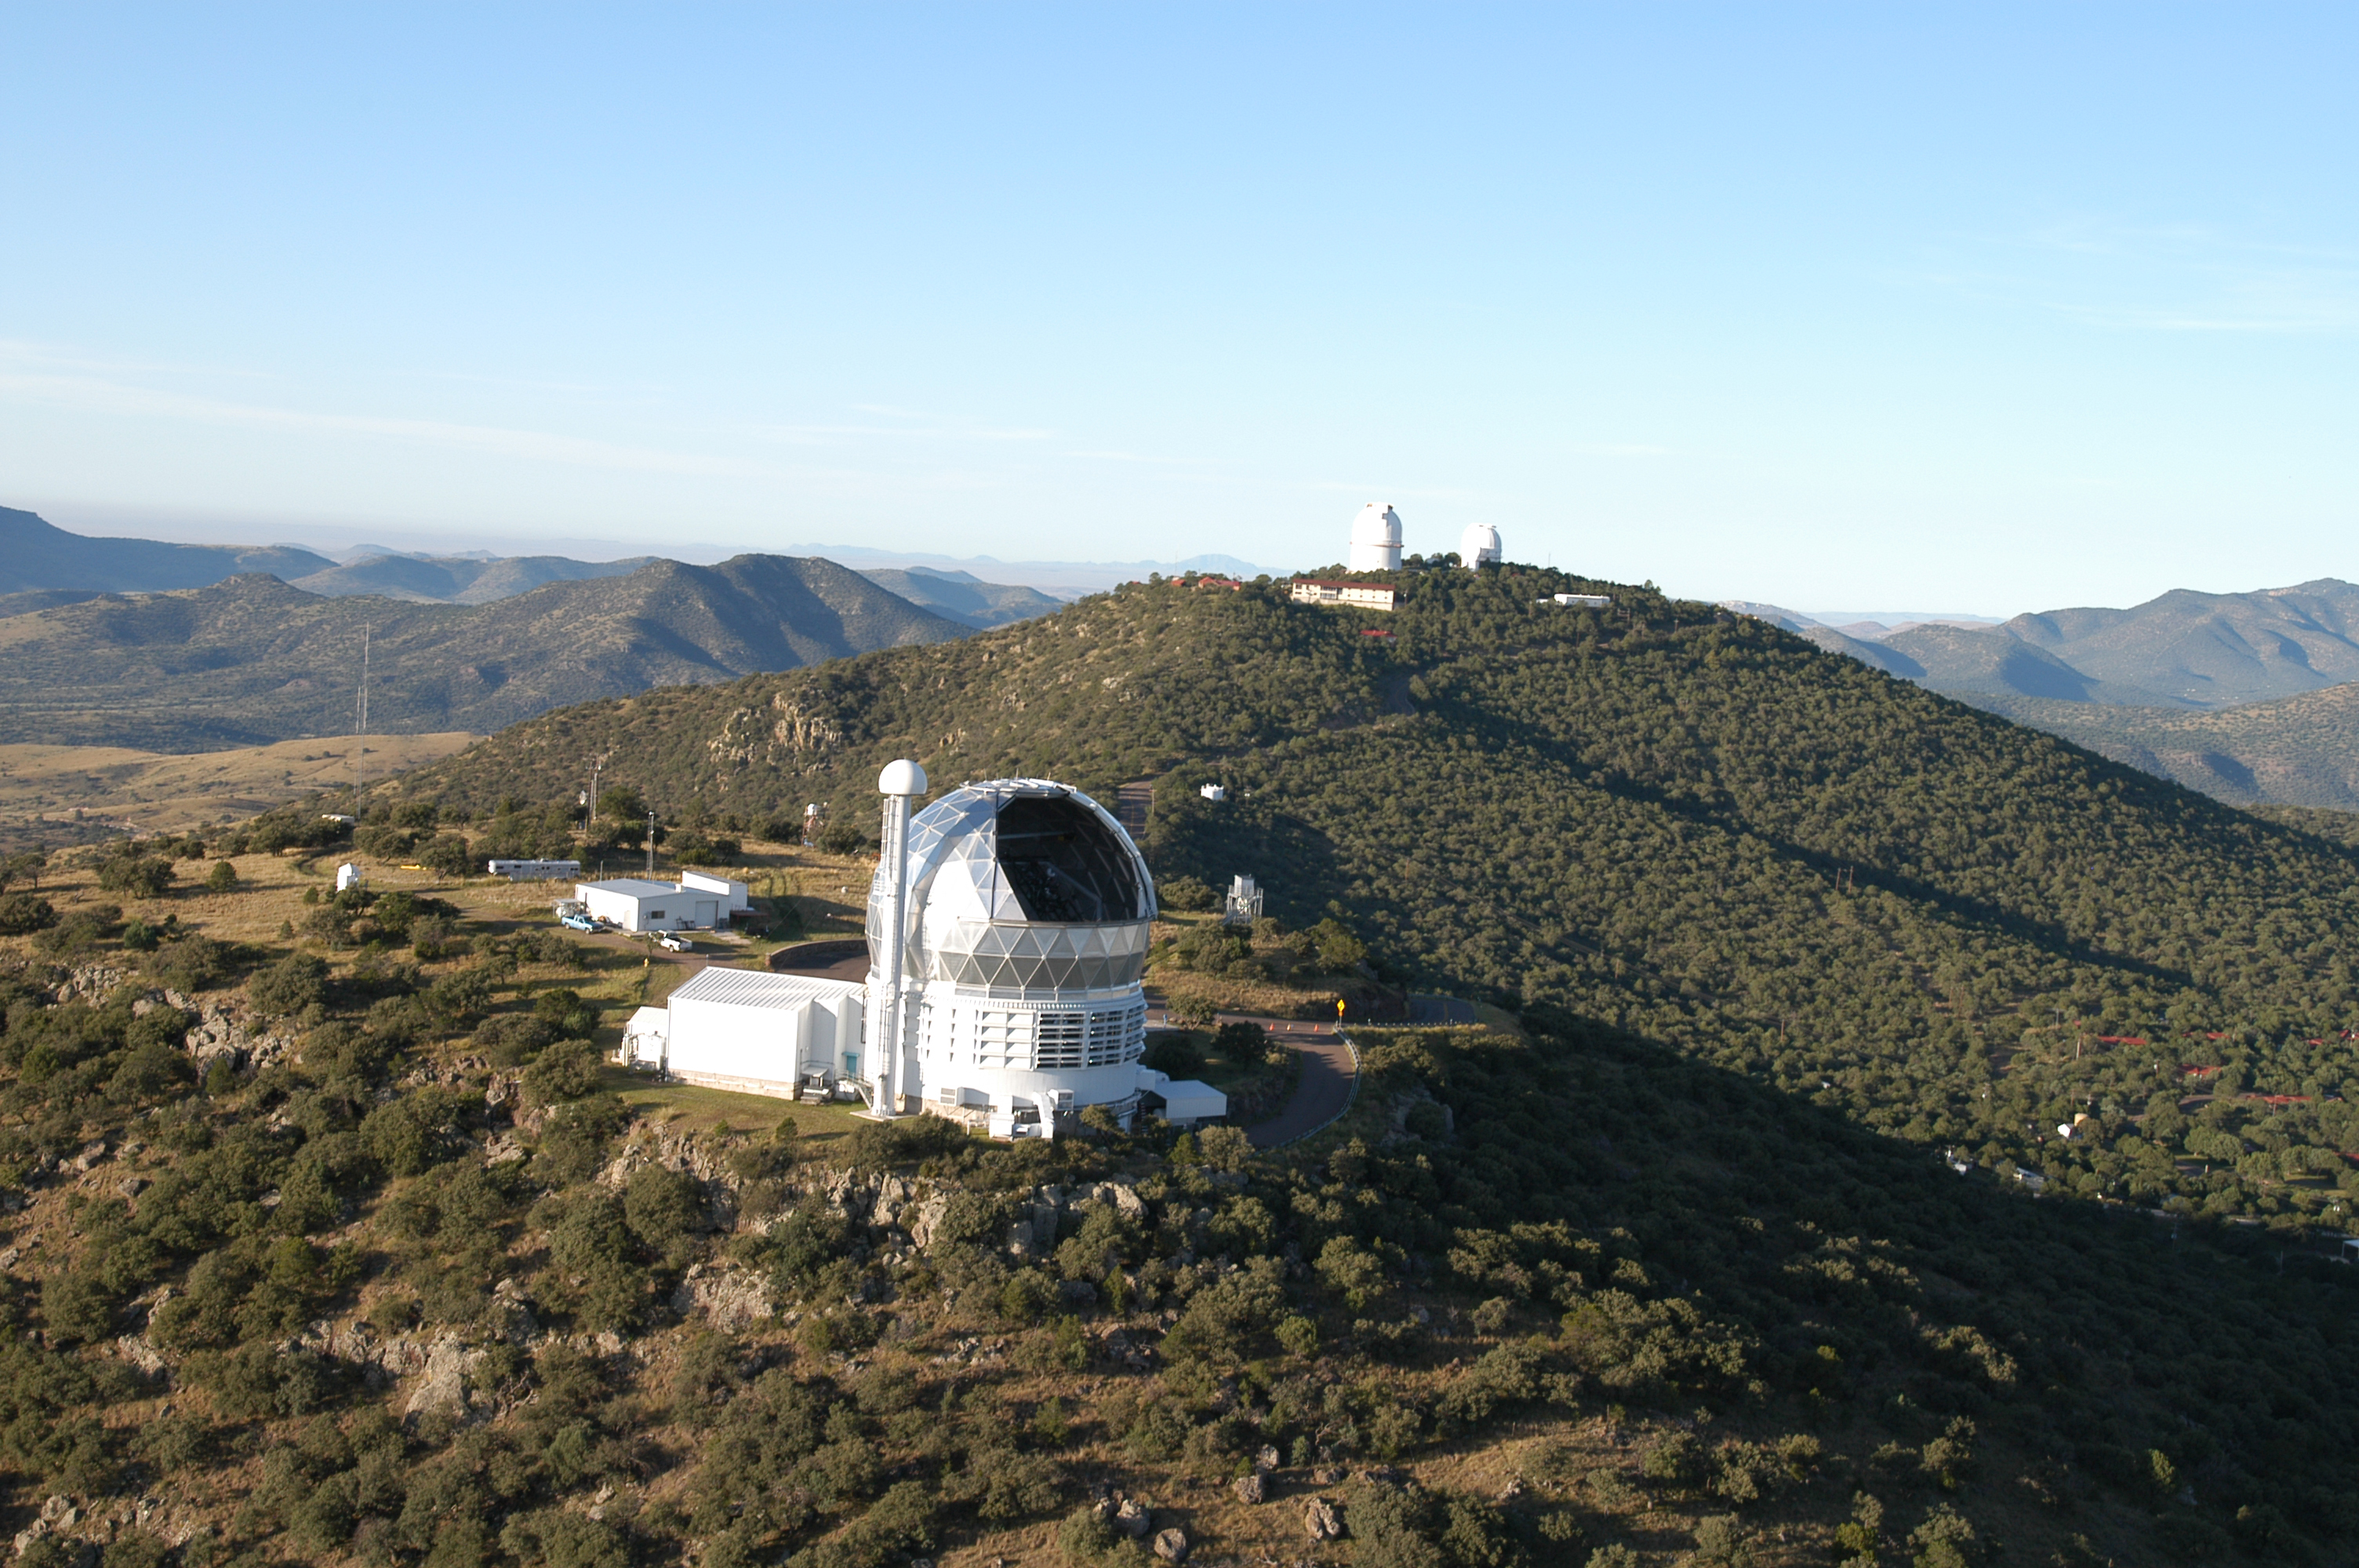
\includegraphics[width=0.8\textwidth]{HETDEX_2212.jpg}
    \end{center}

    \vspace*{-2.5cm}
    \hspace*{7cm}
    \begin{tikzpicture}
        % http://www.usgs.gov/state/state.asp
        \node{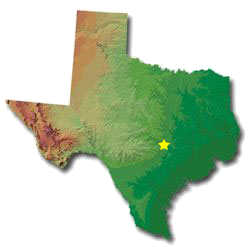
\includegraphics[width=4cm]{TX_transparent_background.png}};
        \draw[color=red,->,very thick] (-2, -1) -> (-1.2, -0.2);
    \end{tikzpicture}

    \begin{textblock*}{\textwidth}(0cm, -1.3cm)
        McDonald Observatory, \SI{10}{\meter} primary

        Every pixel is a spectrograph: \num{36000} spectra
    \end{textblock*}
}


\frame{
    \frametitle{Baryonic Acoustic Oscillations (BAO)}
    \begin{center}
        %http://www.sdss.org/news/releases/20050111.yardstick.html
        \makebox[\textwidth]{
            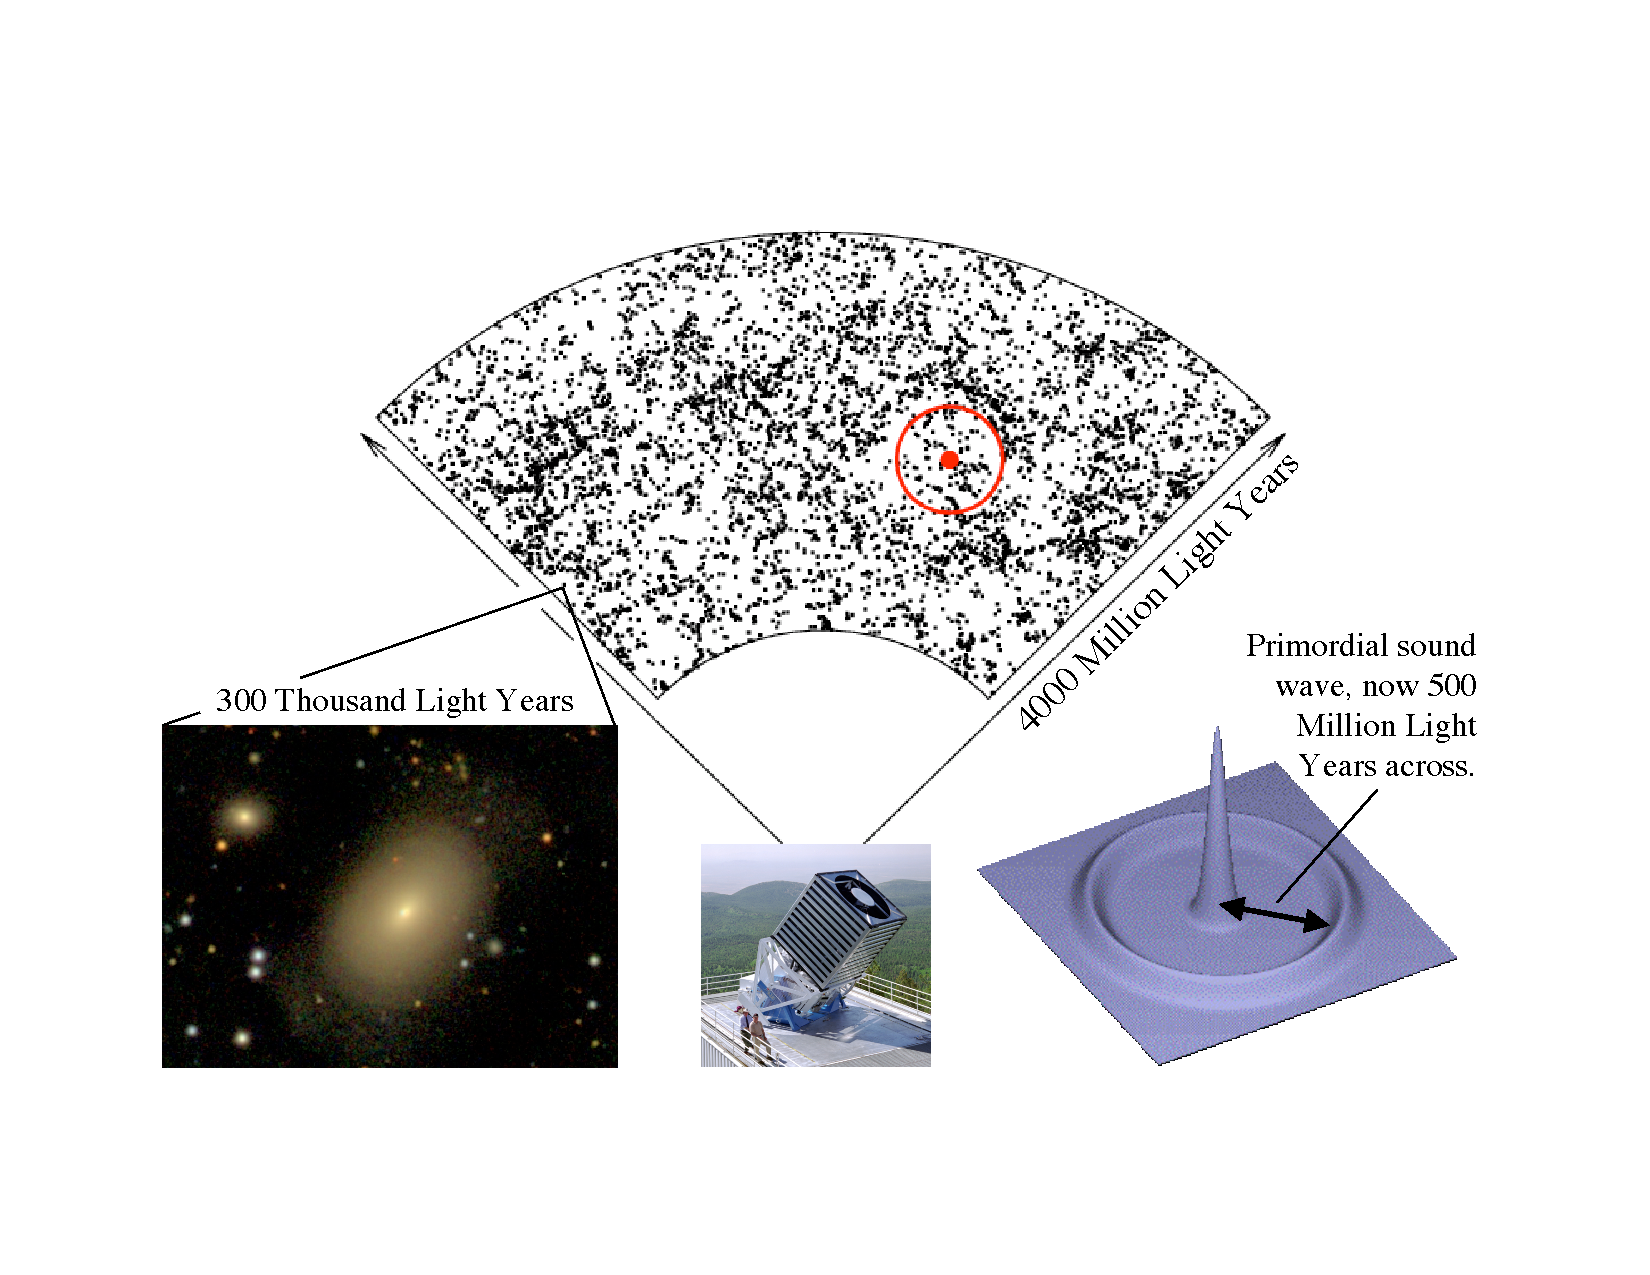
\includegraphics[width=1\textwidth,trim=2cm 3.5cm 2cm 3.5cm,clip]{Acoustic_Figure3.pdf}
        }
    \end{center}
    Sloan Digital Sky Survey out to redshift $z \sim 0.5$.

    Eisenstein \emph{et al.}, 2005.
}


\frame{
    \frametitle{Baryonic Acoustic Oscillations}
    \begin{columns}
        \begin{column}{6cm}
            %https://www.cfa.harvard.edu/~deisenst/acousticpeak/
            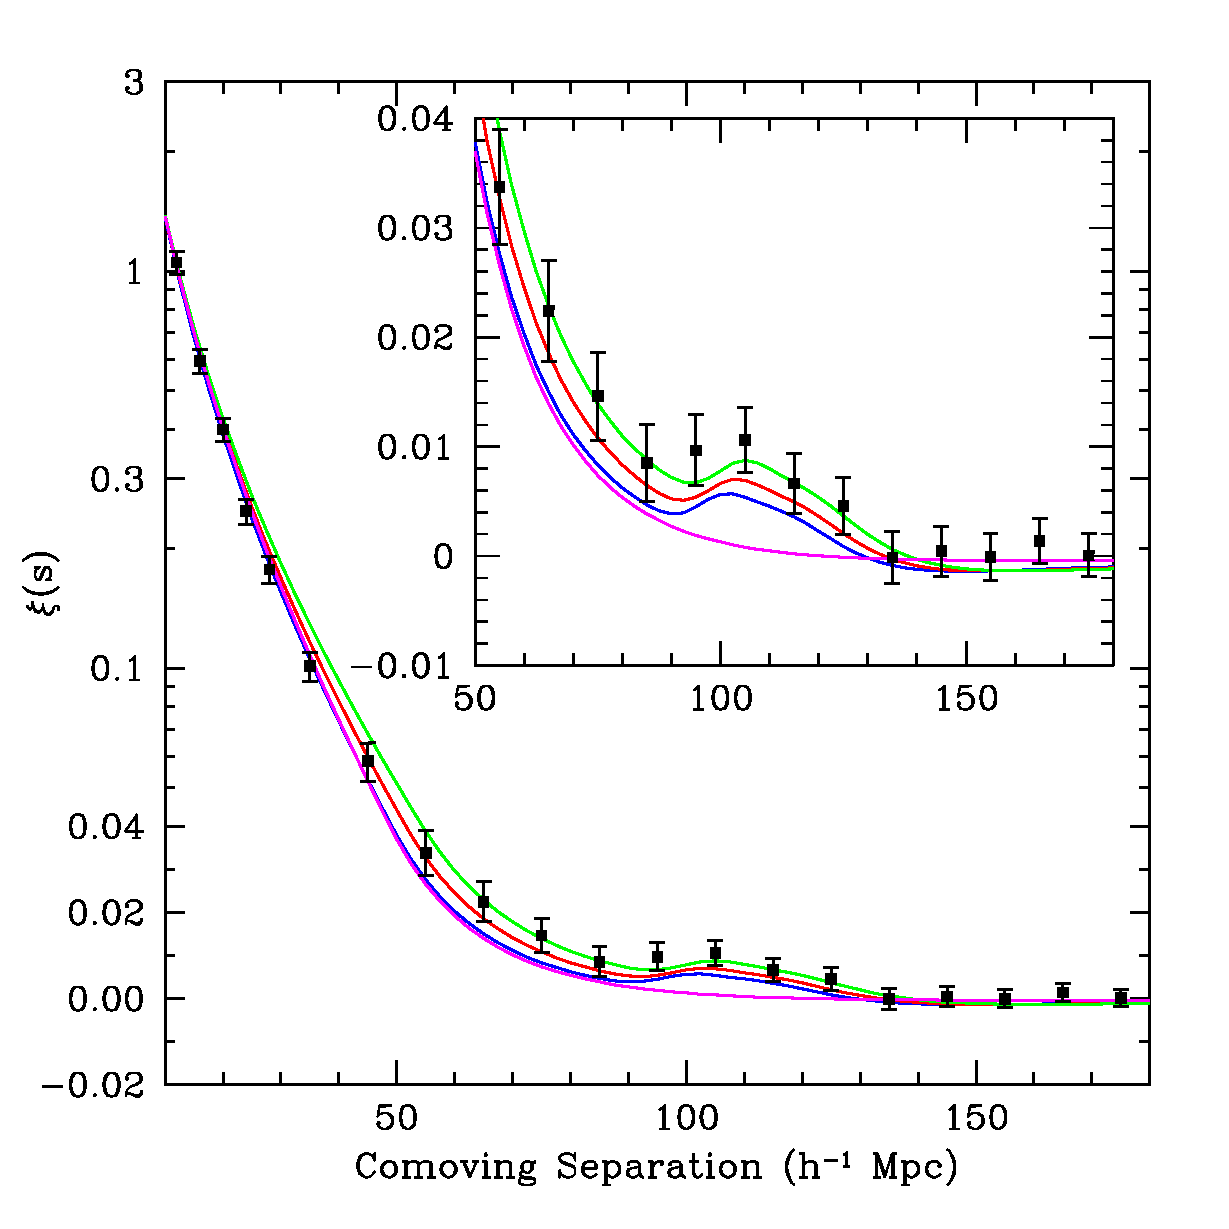
\includegraphics[height=0.7\textheight]{xi_jack.eps}
        \end{column}
        \begin{column}{3cm}
            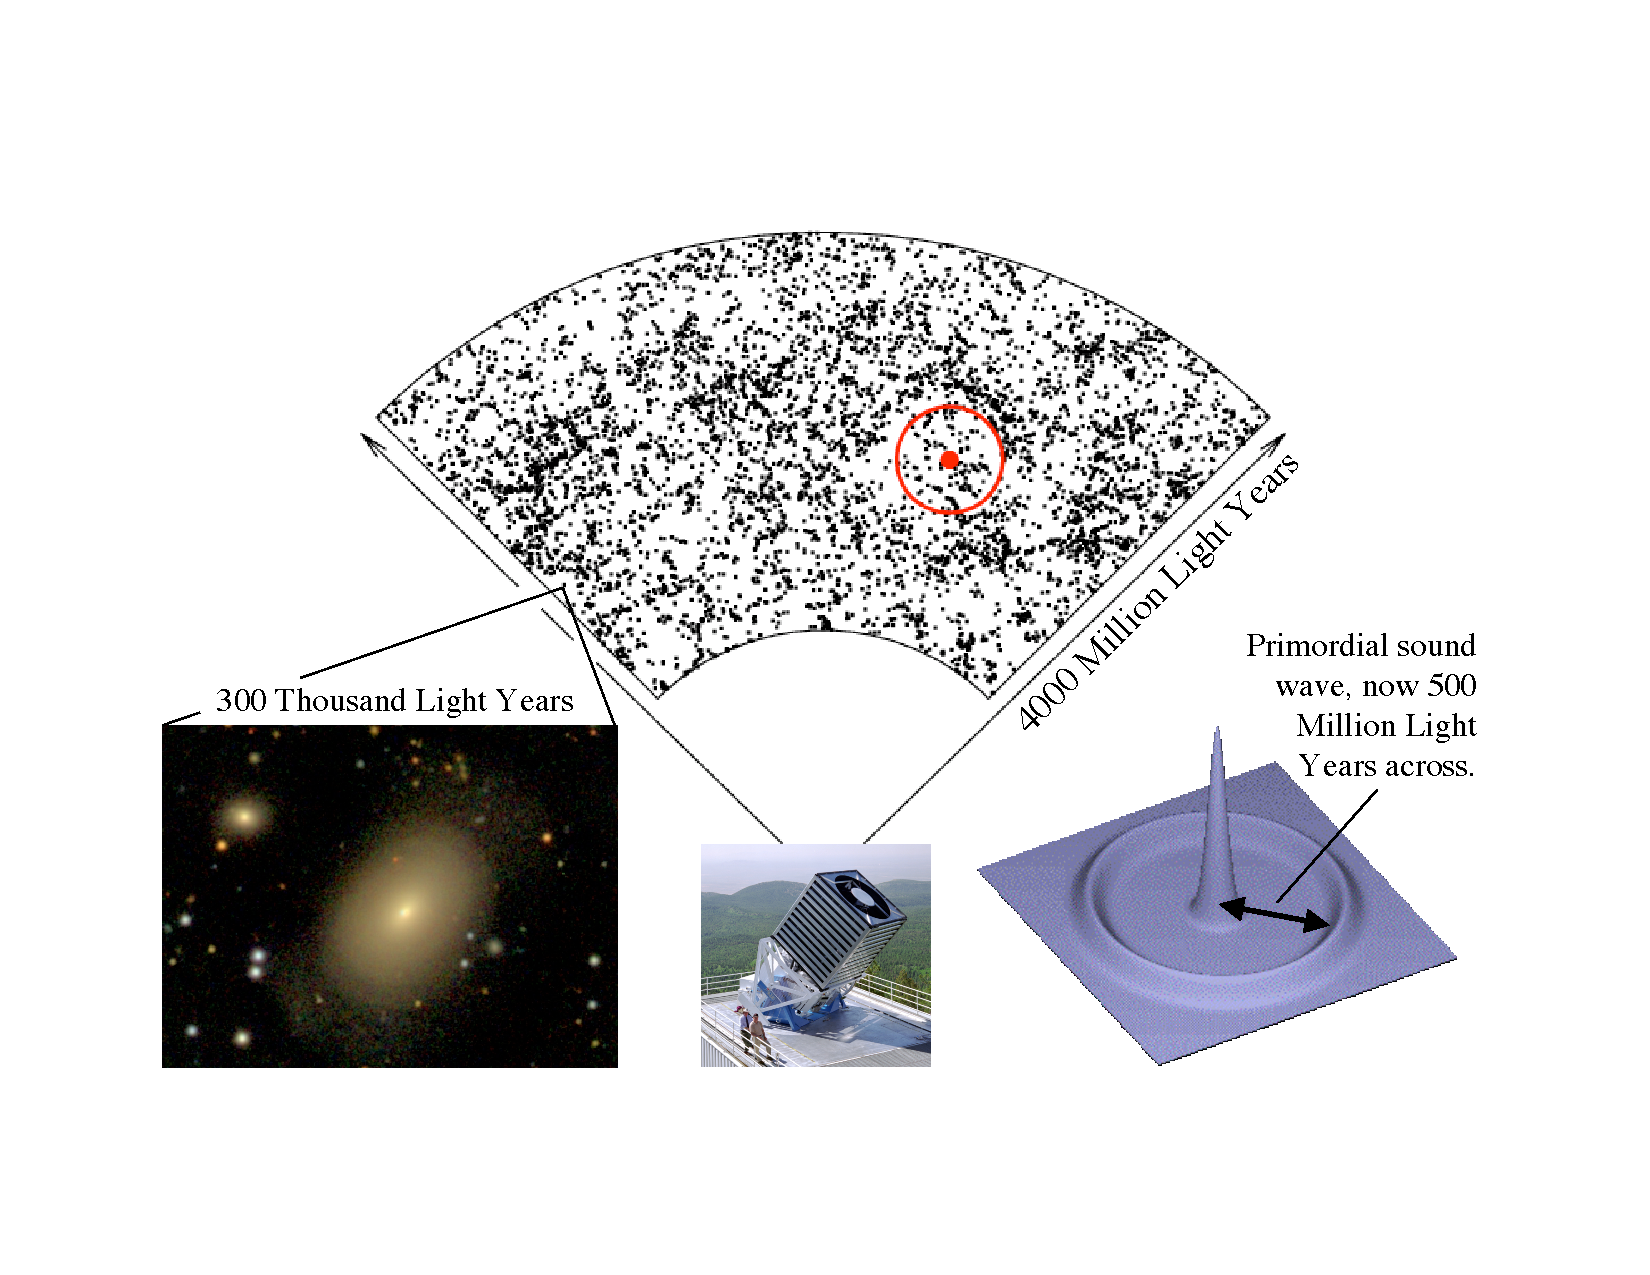
\includegraphics[width=\textwidth,trim=480 100 100 350,clip]{Acoustic_Figure3.pdf}
            \begin{itemize}
                \item Dark Energy
                \item Dark Matter
                \item Baryonic matter
            \end{itemize}
            \begin{itemize}
                \item Oscillations are a standard yardstick
            \end{itemize}
        \end{column}
    \end{columns}
    \medskip
    Eisenstein \emph{et al.}, 2005.
}

\frame{
    \frametitle{HETDEX: How does the view of the yardstick change as a function
    of redshift?}

    \begin{textblock*}{5cm}(7cm, 0cm)
        LAEs: ca. \num{800000} \\
        OII emitters: 1--2~million
    \end{textblock*}

    \begin{tikzpicture}
        % http://astr.ua.edu/keel/galaxies/largescale.html
        \node at (-0.015, 2) {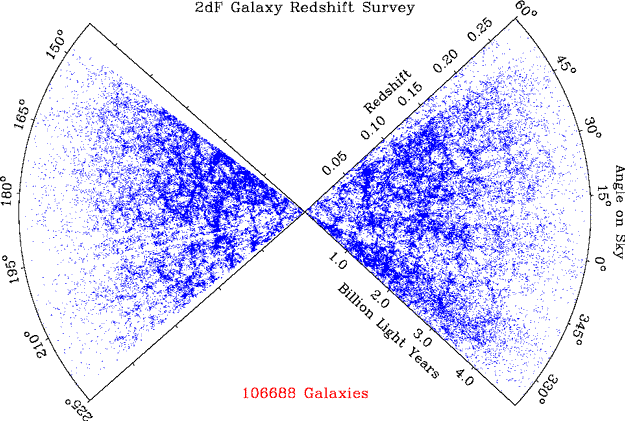
\includegraphics
        [width=4cm,angle=90,clip,trim=305 0 0 0]{2dfjun2000.png}};
        \draw[thick] (0, 0) -- ++(47.5:6cm) arc[start angle=47.5,end angle=132.5,radius=6cm]
        -- cycle;
        \node at (0, 5) {\Huge ???????};
        %
        \pause
        % LAEs
        \draw[<-,color=blue,very thick] (2, 5) -- (4, 5) node[anchor=west] (laes) {Lyman-$\alpha$ emitters};
        \node at (laes) [anchor=105] {
            \begin{minipage}{3cm}
                \medskip
                \raggedright
                LAEs trace the matter distribution at high redshift
            \end{minipage}
        };
        %
        \pause
        % OII emitters
        \draw[<-,color=red,very thick] (0.5, 2) -- (3, 2) node[anchor=west]{Contaminants: OII emitters};
    \end{tikzpicture}

    How does the Hubble \underline{constant} change with time?
}


\frame{
    \frametitle{How to distinguish between LAEs and OII emitters}
    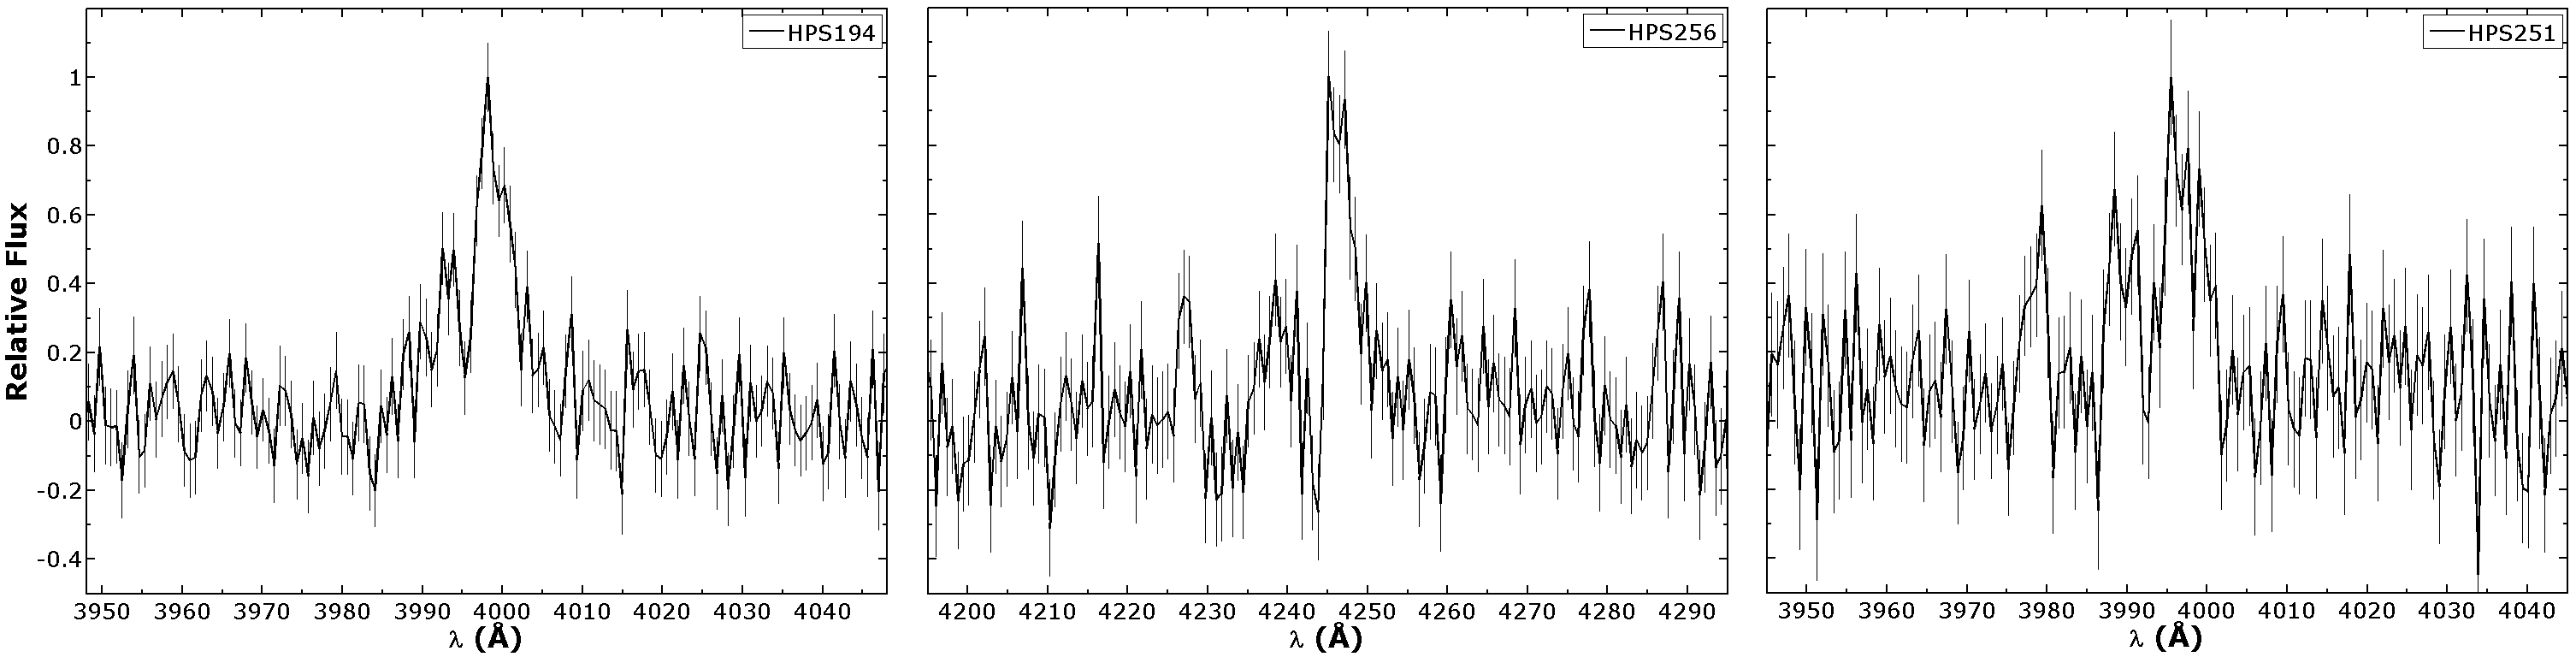
\includegraphics[width=0.5\textwidth,clip,trim=0 0 585 0]{chonis2013/f2.png}

    HETDEX will get something like \num{36000} spectra per exposure.

    Additionally, we will use broadband survey to get continuum flux.

    $\to$ Equivalent width cut:
    \begin{itemize}
        \item LAEs $> \SI{20}{\AA}$
        \item OII $< \SI{20}{\AA}$
    \end{itemize}
    Do Bayesian classification in the future.

    In any case, we need the continuum flux.
}


\frame{
    \frametitle{Project: Simulate a bunch of LAEs and OII emitters, and see how
    well we can distinguish between them}

    \begin{itemize}
        \item Draw RA, Dec, $z$ randomly from power spectrum (done by theorists)
        \item Draw flux randomly from luminosity function
        \item Plop down fake galaxies onto real images (this takes longest!)
    \end{itemize}
    \pause
    \begin{itemize}
        \item Determine flux (using RA, Dec, $z$ given by HETDEX)
        \item YODA (Yet another Object Detection Application)
        \item inherited python code (the horror!)
        \item uses files as communication between methods
    \end{itemize}
}

\frame{
    \frametitle{Problem size}
    \begin{itemize}
        \item $\sim\num{800000}$ LAEs
        \item $\sim2$~million OII emitters
        \item HETDEX will obtain spectra for all of them
        \item still fits in memory (ca.~\SI{500}{\mega B})
        \item should scale mostly linearly
    \end{itemize}

    \begin{itemize}
        \item \path{mpi4py} for embarrassingly easy parallelization
    \end{itemize}
}


\frame{
    \frametitle{Simulation time, Gather time}
    Each thread does its own thing, until we need to gather the results together.
    \begin{center}
        \begin{tikzpicture}
            \begin{loglogaxis}
                [
                    xmax=40000,
                    ymax=800,
                    xlabel=problem size,
                    ylabel=seconds,
                    legend style={draw=none},
                    legend pos=north west
                ]
                \addplot+[blue] table [header=false,x index=0,y index=1] {total_timesshort.dat};
                \addlegendentry{simulation time};
                \addplot+[red] table [header=false,x index=0,y index=1] {gather_timesshort.dat};
                \addlegendentry{gather time};
                \only<2->{
                    \addplot+[blue] table [header=false,x index=0,y index=1] {total_times.dat};
                    %\addlegendentry{simulation time};
                    \addplot+[red] table [header=false,x index=0,y index=1] {gather_times.dat};
                    %\addlegendentry{gather time};
                }
            \end{loglogaxis}
        \end{tikzpicture}
    \end{center}
    $\to$ Astronomical scatter when the network is involved.
}

\frame{
    \frametitle{Many small files}
    \begin{itemize}
        \item IO on \url{lionxv.rcc.psu.edu}:
            \begin{itemize}
                \item network (\$HOME, Infiniband)
                \item disk (\path{/tmp/})
                \item tmpfs (\path{/dev/shm/}, no execute permissions)
            \end{itemize}

            \begin{center}
            \begin{tikzpicture}
                \begin{axis}
                    [
                        height=5cm,
                        width=6cm,
                        symbolic x coords={network,disk,tmpfs},
                        ymin=0,
                        ylabel=seconds,
                    ]
                    \addplot+[error bars/.cd, y dir=both, y explicit]
                    table [header=false,x index=0,y index=1,y error index=3] {write_speed.dat};
                \end{axis}
            \end{tikzpicture}
            \end{center}

            %$\to$ The ancient directives of the UNIX masters are still relevant
            %to this day.

        \item print() statements are slow, especially over the network
    \end{itemize}
}


\appendix


\end{document}


% vim: set sw=4 sts=4 et:
